\newpage
\chapter{Personality}\label{personality}
\pagecolor{gray}\afterpage{\nopagecolor}
\newpage
\pagecolor{gray}\afterpage{\nopagecolor}
blah blah
\newpage

\changepage{9cm}{9.4cm}{-4.7cm}{-4.7cm}{}{-4.5cm}{}{}{}
%\noindent\rule{\textwidth}{\textheight}
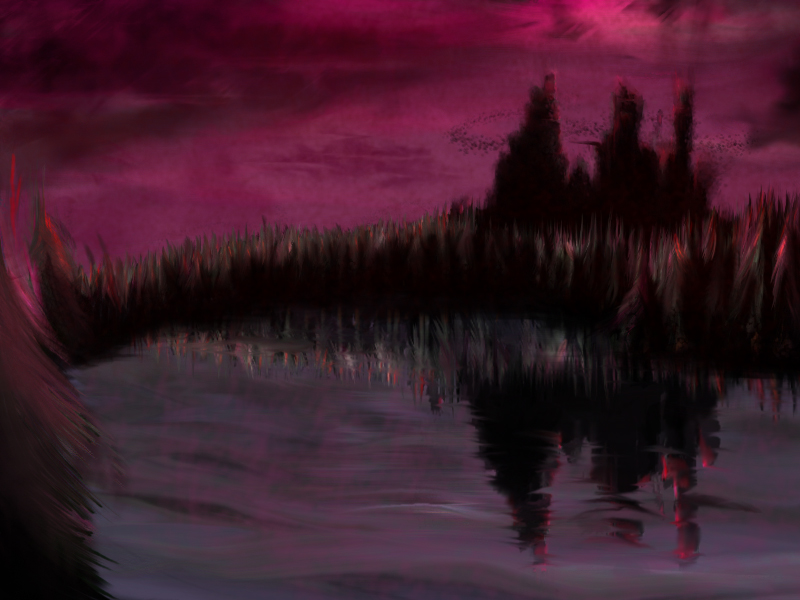
\includegraphics[width=\textwidth,height=\textheight]{Avalonia4}
\newpage

%restoring the standard settings
\changepage{-9cm}{-9.4cm}{4.7cm}{4.7cm}{}{4.5cm}{}{}{}

\begin{multicols}{2}


\subsection{Ethos}
\paragraph{Good}
\paragraph{Evil}
\subsection{Spheres}
Think of your sphere as your birth sign, with power over your deepest thoughts. The reality is that spheres are aspects made manifest by the influences of the esoteric Dread Gates. It is suggested to use Spheres as a way to theme your character and influence his narrative. 

Dont think of spheres as a way to straightjacket your character. They provide no obvious mechanical benefit. It is upto the player to decide how the sphere influences and shapes them. It is possible that multiple spheres are relevant to your character. You have a choice of one sphere and this acts as the primary sphere. The rest would be secondary. 

\begin{tabular}{l|c|r}
    Emotions & Elements & Spiritual \\
    \hline
    Love & Fire & Blasphemy\\
    Hate & Water & Apostacy\\
    Fear & Earth & Despair\\
    Pride & Air & Hatred\\
    Greed & Lightning & Indifference\\
    Lust & Wood & Envy\\
    Apathy & Metal & Sloth\\
    Revenge & Light & Wrath\\
    Honour & Darkness & Gluttony\\
    Glory & Storms & \\
\end{tabular}

\subsection{World View}
\subsubsection{Philosophies}
    \paragraph{Stoicism} "The greatest good was contentment and serenity."
    \paragraph{Hedonism} "Eat, drink and be merry, for tomorrow we die."
    \paragraph{State consequentialism} The moral worth of an action based on how much it contributes to the basic goods of a state.
\paragraph{Ideologies}
\subsection{Politics}
\paragraph{Imperial vs Provincial}
\paragraph{Monarchy vs Republic}
\paragraph{Secular vs Theocratic}
\paragraph{Class conflict}

\end{multicols}